\documentclass[11pt, a4paper]{article}
\usepackage{polski}
\usepackage[utf8]{inputenc}
\usepackage[T1]{fontenc}

\usepackage{graphicx}

\usepackage{amsmath} 

\usepackage{listings}

\usepackage{color}

\usepackage{marvosym}

\usepackage{geometry}
\usepackage{float}
\usepackage{booktabs}
\usepackage{multirow}
\usepackage{titlesec}
\usepackage{hyperref}

\geometry{margin=1.2in}
\usepackage[final]{pdfpages}

\newcommand{\fbi}{\leavevmode{\parindent=1em\indent}}

\definecolor{dkgreen}{rgb}{0,0.6,0}
\definecolor{gray}{rgb}{0.5,0.5,0.5}
\definecolor{mauve}{rgb}{0.58,0,0.82}

\lstset{
	frame=tblr,
	language=R,
	aboveskip=3mm,
	belowskip=3mm,
	showstringspaces=false,
	columns=flexible,
	basicstyle={\small\ttfamily},
	numbers=left,
	numberstyle=\tiny\color{gray},
	keywordstyle=\color{blue},
	commentstyle=\color{dkgreen},
	stringstyle=\color{mauve},
	breaklines=true,
	mathescape=false,
	breakatwhitespace=true,
	tabsize=3
}

\renewcommand\lstlistingname{Listing}

\titleclass{\subsubsubsection}{straight}[\subsection]
\newcounter{subsubsubsection}[subsubsection]
\renewcommand\thesubsubsubsection{\thesubsubsection.\arabic{subsubsubsection}}
\renewcommand\theparagraph{\thesubsubsubsection.\arabic{paragraph}}

\titleformat{\subsubsubsection}
  {\normalfont\normalsize\bfseries}{\thesubsubsubsection}{1em}{}
\titlespacing*{\subsubsubsection}
{0pt}{3.25ex plus 1ex minus .2ex}{1.5ex plus .2ex}

\makeatletter
\renewcommand\paragraph{\@startsection{paragraph}{5}{\z@}%
  {3.25ex \@plus1ex \@minus.2ex}%
  {-0em}%
  {\normalfont\normalsize\bfseries}}
\renewcommand\subparagraph{\@startsection{subparagraph}{6}{\parindent}%
  {3.25ex \@plus1ex \@minus .2ex}%
  {-1em}%
  {\normalfont\normalsize\bfseries}}
\def\toclevel@subsubsubsection{4}
\def\toclevel@paragraph{5}
\def\toclevel@paragraph{6}
\def\l@subsubsubsection{\@dottedtocline{4}{7em}{4em}}
\def\l@paragraph{\@dottedtocline{5}{10em}{5em}}
\def\l@subparagraph{\@dottedtocline{6}{14em}{6em}}
\makeatother

\setcounter{secnumdepth}{4}
\setcounter{tocdepth}{4}

\hypersetup{pageanchor=false}

\setlength\parindent{3pt}

\renewcommand{\labelenumi}{\alph{enumi}.} 

\date{\today}

\begin{document}

\begin{titlepage}

\newcommand{\HRule}{\rule{\linewidth}{0.5mm}} 
\center 

\textsc{\LARGE Politechnika Wrocławska}\\[1.5cm] 
\textsc{\Large Inteligencja Obliczeniowa i jej zastosowania}\\[0.5cm] 
\HRule \\[0.5cm]
{ \huge \bfseries Badanie algorytmu genetycznego z zakresu optymalizacji globalnej dla wybranych funkcji testowych}\\[0.5cm] 
\HRule \\[1.6cm]
 
\begin{minipage}{0.4\textwidth}
\begin{flushleft} \large
\emph{Autorzy:}\\
Paweł  \textsc{Andziul} 200648 \\
Marcin  \textsc{Słowiński} 200638 \\
\end{flushleft}
\end{minipage}
~
\begin{minipage}{0.4\textwidth}
\begin{flushright} \large
\emph{Prowadzący:} \\
dr hab. inż. Olgierd \textsc{Unold}, prof. nadzw. PWr
\end{flushright}
\end{minipage}\\[4cm]

\vfill 
{\large 5 kwietnia 2017}\\[3cm] 

\end{titlepage}

\tableofcontents

\newpage
\section{Wprowadzenie}
\paragraph{}
Wstęp

\subsection{Opis zadania projektowego}



\subsection{Środowisko testowe i narzędzia}

\newpage
\section{Implementacja}

\lstinputlisting[label="lst:skryptGlowny",caption=Skrypt w języku R wykorzystany do badań,firstline=1,lastline=82]{./assets/skrypt_lab12.R}


\subsection{Parametryzacja skryptu}

\newpage
\section{Przebieg badań}
\paragraph{}
Akapit

\subsection{Funkcja Ackleys (wariant 2D)}
\paragraph{}
Test

\subsection{Funkcja Ackleys (wariant 3D)}
\paragraph{}
Test

\fbi
Na ilustracji (rys.~\ref{fig:ackleys3dwykres}) przedstawiono wykres omawianej funkcji.

\begin{figure}[H]
	\begin{center}
		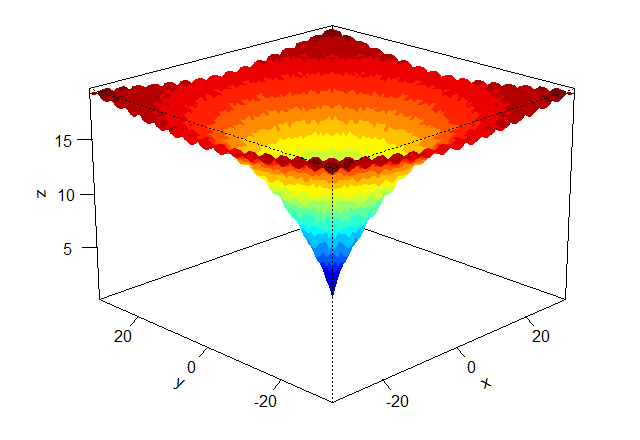
\includegraphics[width=0.9\textwidth]{./assets/ackleys3d.png} % 
		\caption{Wykres funkcji Ackleys (d=3)}
		\label{fig:ackleys3dwykres}
	\end{center}
\end{figure}

\begin{figure}[H]
	\begin{center}
		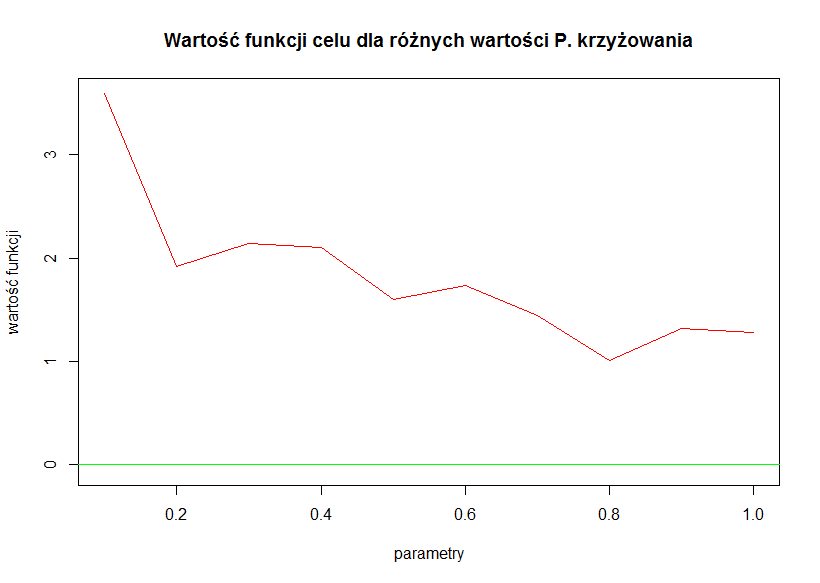
\includegraphics[width=0.9\textwidth]{./assets/ackleys3dkrzyzowanie.png} % 
		\caption{Wartość znalezionego minimum funkcji w zależności od P. krzyżowania}
		\label{fig:ackleys3dkrzyzowanie}
	\end{center}
\end{figure}

\subsection{Funkcja Branin (wariant 3D)}
\paragraph{}
Test

\subsection{Funkcja Schwefel (wariant 3D)}
\paragraph{}
Minimum -837,9658 w punkcie (420,9687; 420,9687).

\newpage
\section{Podsumowanie}
\paragraph{}
Test

\fbi
Akapit






\newpage
\begin{thebibliography}{40}

\bibitem{test1}
Artur Suchwałko “Wprowadzenie do R dla programistów innych języków” https://cran.r-project.org/doc/contrib/R-dla-programistow-innych-jezykow.pdf

\end{thebibliography}

\end{document}